\documentclass[a4paper]{article}

\usepackage[swedish]{babel}
\usepackage[latin1]{inputenc}
\usepackage{amssymb}
\usepackage{framed}
\usepackage{graphicx}


\setlength{\parindent}{0pt}
\setlength{\parskip}{3ex}

\begin{document}

\begin{center}
  {\large Artificial Neural Networks and Deep Architectures, DD2437}\\
  \vspace{7mm}
  {\huge Short report on lab assignment 1\\[1ex]}
  {\Large Classification with a single-layer perceptron}\\
  \vspace{8mm}  
  {\Large Hasan, Rakin Ali and Steinar Logi \\}
  \vspace{4mm}
  {\large January 22, 2024 \\}
\end{center}

\section{Main objectives and scope of the assignment \normalsize}
The main objective with this assignment is to familiarize ourselves with the perceptron learning rule and the delta learning rule along with batch versus sequential learning method. 
Our major goals in the assignment were  
\begin{itemize}
\item Implement and explore the perceptron learning rule for simple classification tasks
\item Implement and explore the delta learning rule for simple classification tasks 
\item Explore how the perceptron and delta learning rule performs on linearly separable data compare to a dataset that is not linearly separable
\item Explore how the bias affects the convergence of the delta learning algorithm
\end{itemize}

This assignment was scoped on the delta and perceptron learning rule. For the delta rule we used batch learning and sequential learning and for the delta rule we only used sequential learning. The limitations were the different learning rate

\section{Methods} This lab was conducted three separate times as we did not collaborate when writing the code. We all did the code separately then compared our results. The code was written in Jupyter notebook and regular python v3.9 file. We all drew the same conclusions on our results however got different graphs. Numpy function and matplot were the only libraries used.  \\

\section{Results and discussion}
\subsection{Classification with a single-layer perceptron}

\begin{figure}
    \centering
    \includegraphics{}
    \caption{Caption}
    \label{fig:enter-label}
\end{figure}
\begin{figure}
    \centering
    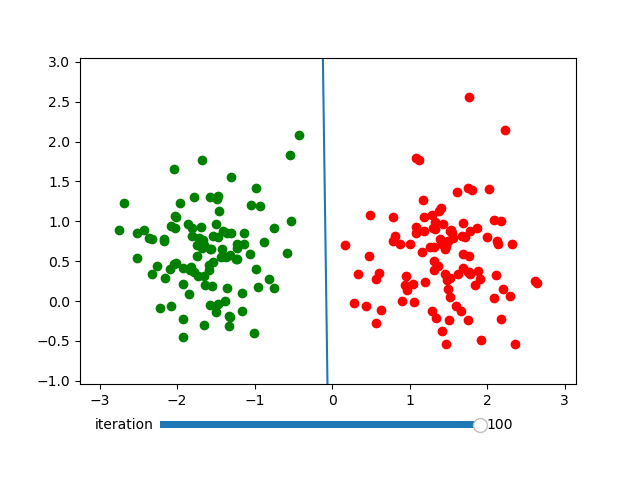
\includegraphics{Labs/Lab 1/Lab 1a/Results/Delta-linear-seperable.png}
    \caption{Delta rule}
    \label{fig:Delta Rule}
\end{figure}

\subsection{Classification of data that are not linearly separable\textit{(ca.1.5-2 pages)}}
Let's first try to do regular classification. Here the bias is 

\begin{figure}
    \centering
    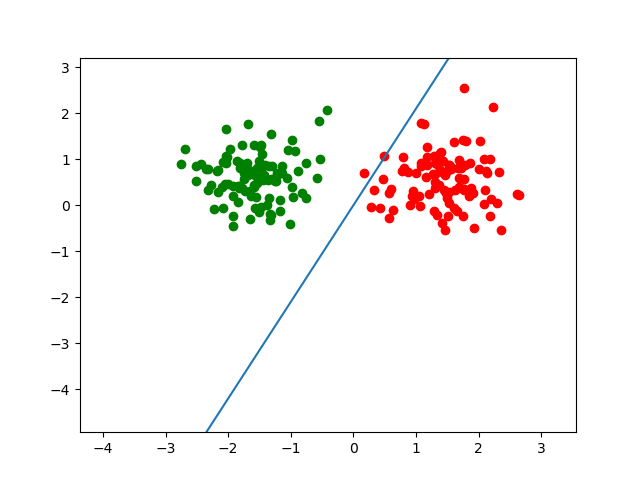
\includegraphics{Labs/Lab 1/Lab 1a/Results/perceptron-linearly-seperable.png}
    \caption{Perceptron}
    \label{fig:Perceptron-withBias}
\end{figure}

\section{Final remarks \normalsize{\textit{(ca. 0.5 page)}}} \textbf{Rakin Ali }
\textit{Please share your final reflections on the lab, its content and your own learning. Which parts of the lab assignment did you find confusing or not necessarily helping in understanding important concepts and which parts you have found interesting and relevant to your learning experience? \\
Here you can also formulate your opinion, interpretation or speculation about some of the simulation outcomes. Please add any follow-up questions that you might have regarding the lab tasks and the results you have produced.}

\end{document}
